
\documentclass[twocolumn,10pt]{article}

\usepackage{balance}
\usepackage[margin=1.0in]{geometry}
\usepackage{graphicx}
\usepackage{ifpdf,theorem,tabularx,multirow}

\newcommand{\ie}{{\em i.e.,}~}
\newcommand{\eg}{{\em e.g.,}~}

\begin{document}
\title{Big Data Analysis Exploiting Genome Similarity\\ Qualifying Exam}
\author{Kristal Curtis}
\date{Dec. 13, 2012}
\maketitle

\abstract

\section{Introduction} 

\section{Improving Alignment with SNAP}

\section{The Similarity Problem}

After implementing the basic SNAP algorithm, we explored how various properties of its search parameters and input data affect its speed and accuracy.  Through this process, we discovered that the main obstacle to both speed and accuracy in alignment is the \textit{similar regions} in the genome.  In what follows, we discuss our observations of how similar regions impact SNAP's performance.  Then, we describe a method for identifying the similar regions, as well as some insights into their characteristics.  We also discuss how we plan to exploit genome similarity throughout the pipeline to improve speed and accuracy of variant calling.

% could also be "Motivation"
\subsection{Observations}

One of our goals following the development of SNAP was to determine the impact of its various parameters on its speed and accuracy.  By accuracy, I mean to encompass both \% aligned and \% error.  Thus, we performed a parameter sweep.  We observed that the only parameter that significantly impacted SNAP's performance was \(h_{max}\), which is the maximum number of genome locations to which a seed could match and still be considered by SNAP.  Seeds occurring at more positions in the genome than \(h_{max}\) are ignored by SNAP, to avoid spending undue time attempting to match reads that are unlikely to be matched uniquely.

Figure \ref{fig:maxHits} shows the results of this parameter sweep.  As we increase \(h_{max}\), the alignment accuracy improves, \ie we are able to align more reads while making fewer errors.  However, this comes at a significant cost to throughput.  The interesting thing about this result is that while you might think that a read that contains popular seeds cannot be uniquely mapped, what we actually observe is that these reads that map to lots of locations actually can be mapped uniquely if we check enough locations, hence the improvement to \% aligned.

\begin{figure*}
\centering
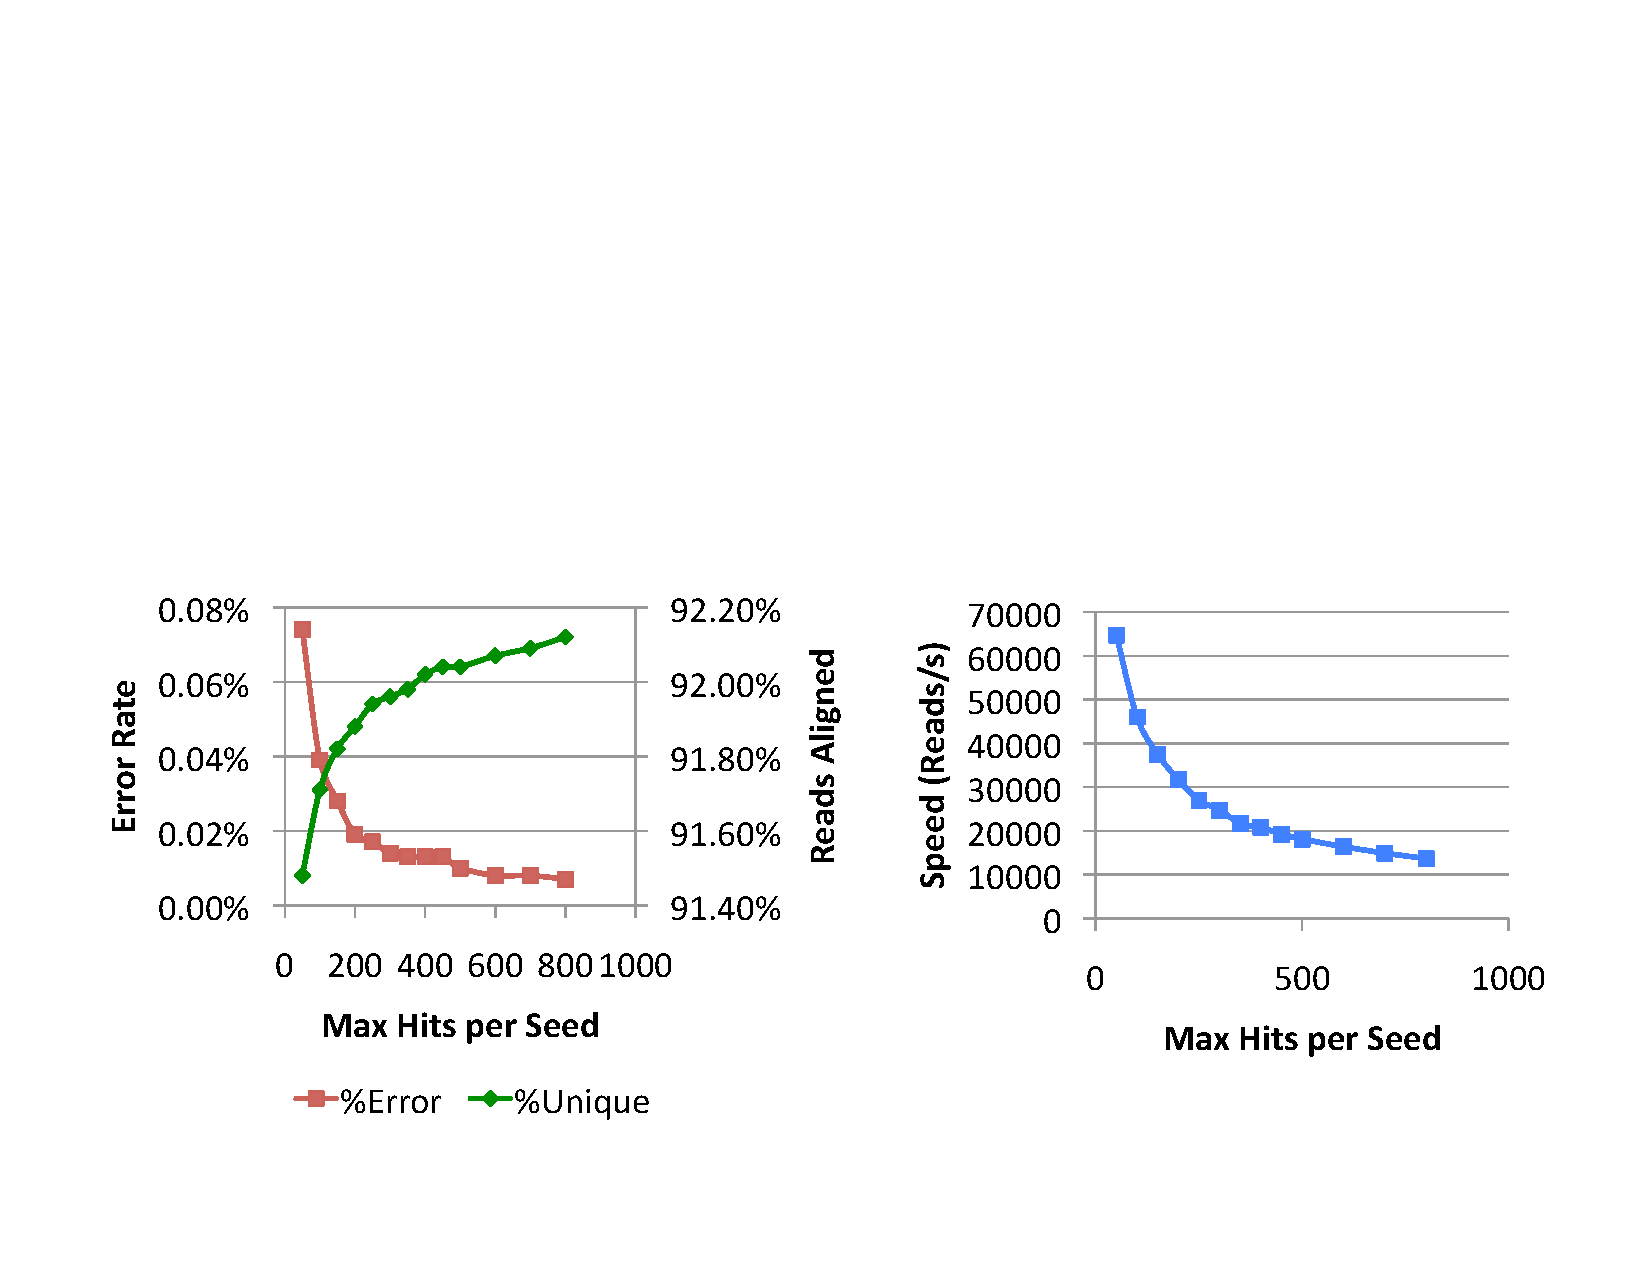
\includegraphics[scale=0.6]{maxHits.pdf}
\caption{Accuracy improves as we increase \(h_{max}\), the number of locations we check per seed, but throughput suffers.}
\label{fig:maxHits}
\end{figure*}

We discovered that this is due to the repetitive nature of the genome.  Exact duplicates are not as confounding, since if the problem were just that there are too many exact duplicates, increasing \(h_{max}\) would not result in any increase in \% aligned, since it would be impossible to find a unique mapping location no matter how many locations SNAP considers.  The difficulty here is caused by near duplicates, which we refer to as \textit{similar regions}.  The presence of near duplicates means that in many cases, it actually is possible to find a unique alignment for a read that contains popular seeds, due to slight differences between the similar regions.  Thus, there is a benefit to checking many locations per read, even though it is expensive.

To confirm our intuition that similar regions are presenting a significant obstacle to alignment performance, we did a simple experiment.  We aligned one million reads, simulated from the whole genome, with SNAP.  Then, for the reads which SNAP aligned incorrectly, we checked whether the read belonged to a cluster.  How the clusters were located will be described in Section \ref{section:identifyingSimilarRegions}.  Our findings were surprising; out of the 227 errors that SNAP made, 195 (86\%) were in clusters.  For reference, only 8\% of the positions in hg19 belong to a cluster.  Therefore, the clusters, though making up a small fraction of the genome, make a huge impact on alignment performance.  Thus, it is essential to improve the handling of these reads in order to improve alignment performance.

\begin{figure*}
\centering
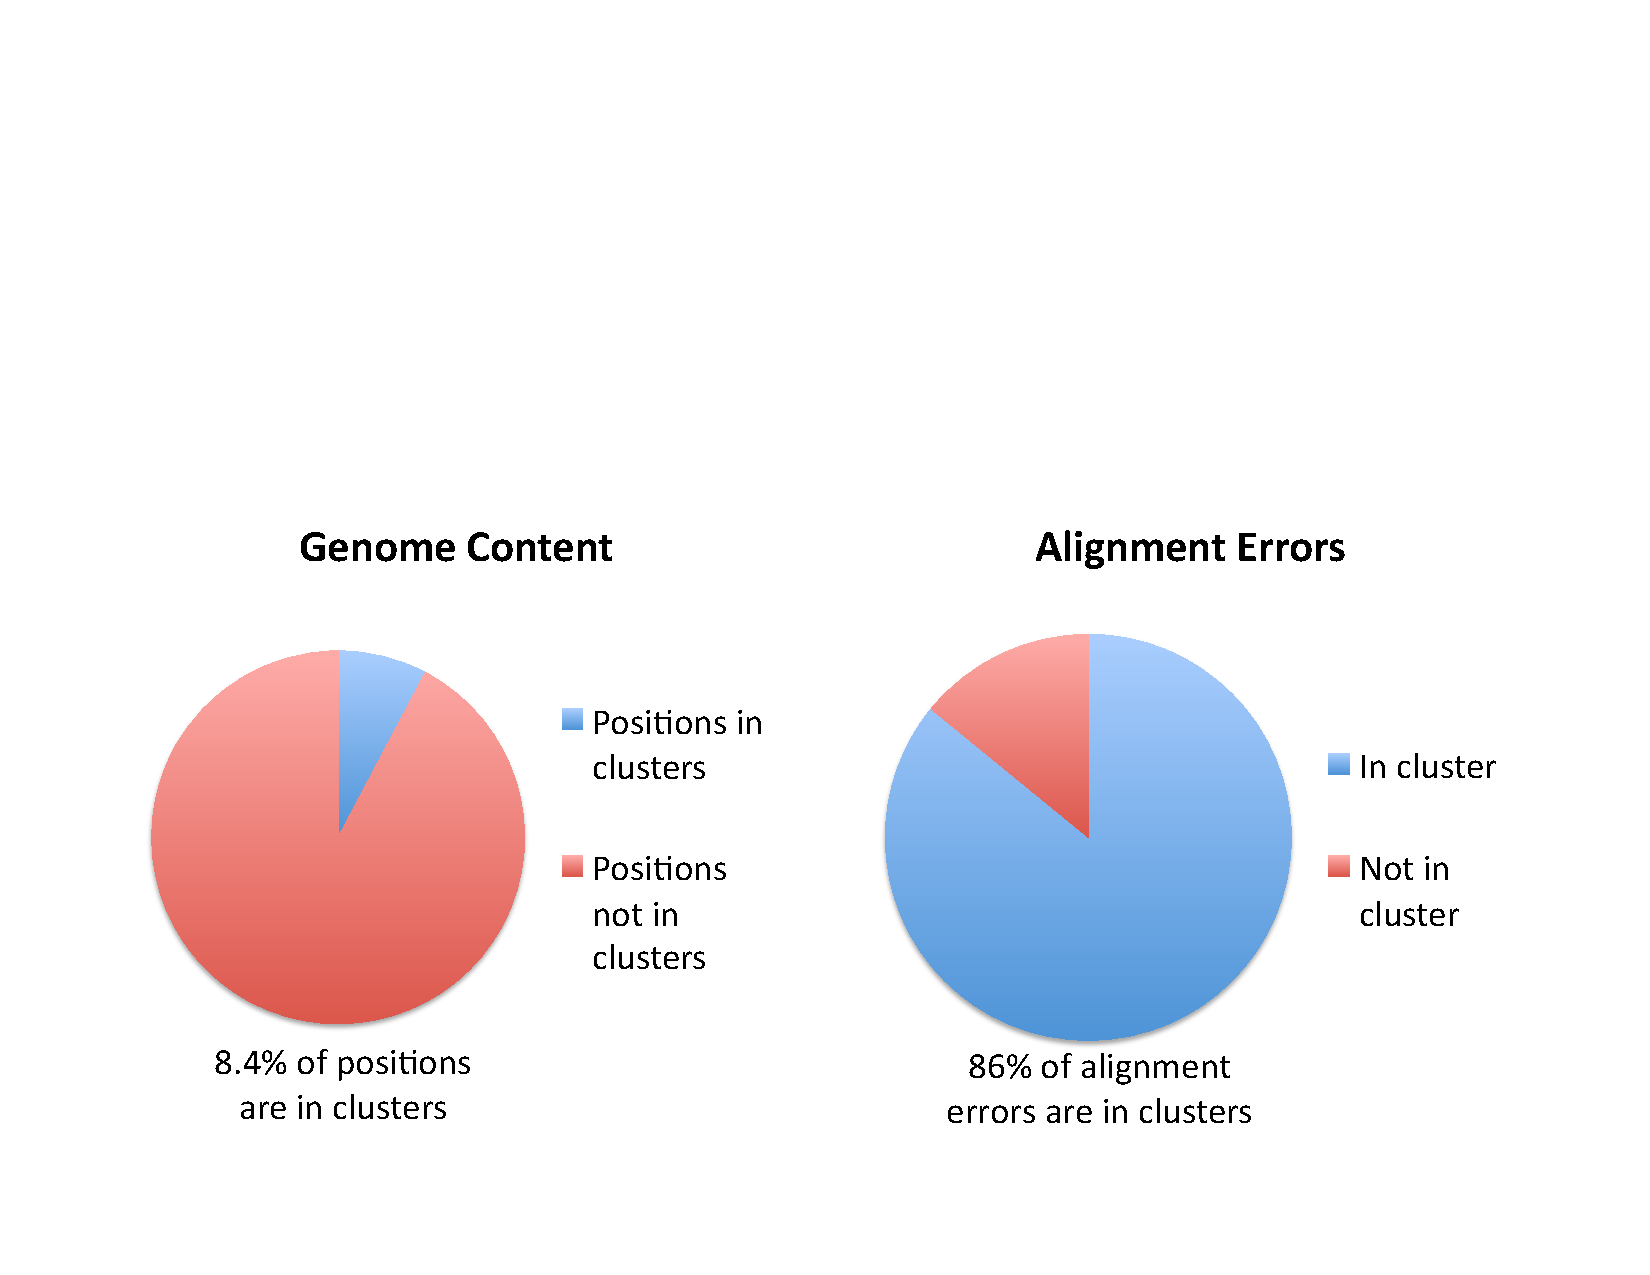
\includegraphics[scale=0.6]{errorsInClusters.pdf}
\caption{Despite the fact that a small fraction of the genome belongs to a cluster, a significant fraction of alignment errors occur in clusters.}
\label{fig:errorsInClusters}
\end{figure*}

\subsection{Identifying Similar Regions}
\label{section:identifyingSimilarRegions}

% talk about how union find works
The straightforward approach to find clusters would be to create a graph where the nodes are the substrings in the genome and there is an edge between any two nodes that are sufficiently similar.  Then, the clusters correspond to the connected components of this graph.  However, since there are over 3 billion substrings of length 100, the length of the short reads we are using, both building this graph and then the subsequent step to find the connected components are very expensive.  Therefore, we chose to approximate this approach by using the well-known \textit{union-find algorithm}.  In union-find, each substring starts in its own cluster.  Then, whenever two substrings are sufficiently similar, we merge the two clusters.  The output of this process is similar to the connected components of the graph identified by the straightforward approach; however, the union-find implementation is much more efficient.  In order to determine which clusters to merge, we use the SNAP index to find all locations to which a substring's seeds map.  Thus, we avoid doing the full \(N \times N\) comparison of all the substrings in the genome.

% talk about how I used Spark for the implementation
Though the union-find algorithm is more efficient than the na\"{\i}ve connected components approach, it is non-trivial to implement it so that it will run in a practical amount of time on the whole genome.  From the initial version that ran on chromosome 22 to the current version that runs on the full hg19, several implementation changes were needed.  The main change was going from a serial implementation to a parallel version using Spark \cite{Zaharia:2012}.  The parallel version finds clusters in each partition, and then it merges the clusters to produce clusters that are present in the genome overall (Figure \ref{fig:sparkUnionFind}).  Once we had a parallel implementation, we had to do several tricks to make it scale, such as changing the partitioning scheme, using a feature of Spark called accumulators to avoid storing intermediate results, and changing the representation of genome locations so that they could be stored in 4-byte integers instead of 8-byte longs.  These changes were mainly motivated by saving memory.

\begin{figure*}
\centering
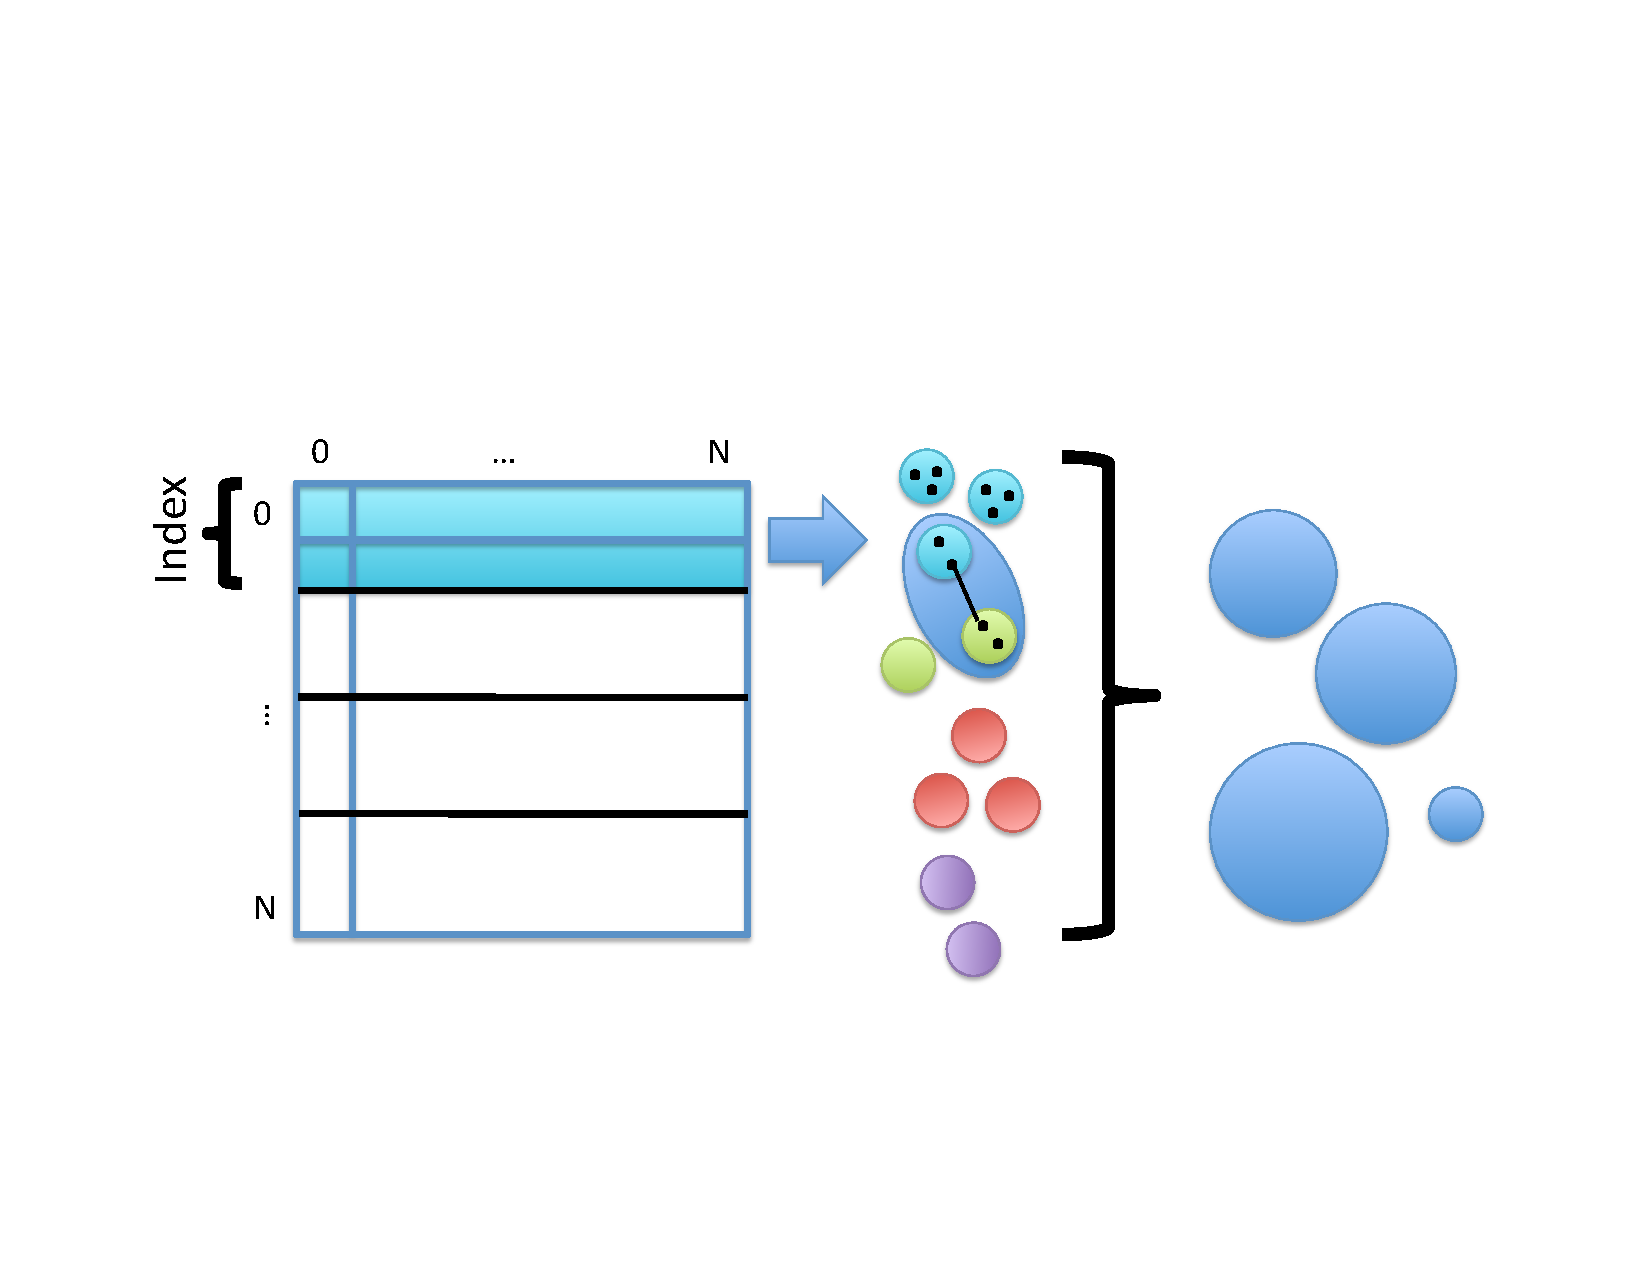
\includegraphics[scale=0.6]{sparkUnionFind.pdf}
\caption{Union-find implementation via Spark.  Parallel implementation involves partitioning the genome.  We find clusters in each partition separately and then merge them to obtain clusters in the genome overall.}
\label{fig:sparkUnionFind}
\end{figure*}

% talk about the pros/cons of this approach
Compared to other approaches to clustering the genome (see Section \ref{section:clusteringTheGenome}), our approach has several advantages.  First, because our approach is driven by the characteristics of the short reads themselves, rather than being motivated by a more biological desire to better understand the repeat characteristics of the genome, our problem is more constrained.  Many of the previous approaches to clustering the genome attempt full generality, without imposing any constraints on repeat length, and allowing many only marginally related substrings to belong to the same repeat family in the interest of reducing the number of repeat families to enhance interpretability.  However, this results not only in algorithms that are very complicated and computationally expensive but also in output that is difficult to utilize for short-read processing.  Our more constrained problem, where we fix the length of any substrings considered to be the same as that of the short reads, is simpler to tackle and is therefore more amenable to an efficient algorithm.  
% still need to talk about cons

% talk about the results

\subsection{Vision for Exploiting Similar Regions}

\section{Exploiting Similarity in Alignment}

\section{Exploiting Similarity throughout the Pipeline}

\section{Related Work}

\subsection{Alignment}

\subsection{Clustering the Genome}
\label{section:clusteringTheGenome}

\section{Research Timeline}

% Paragraph on finishing the SNAP paper with cluster-informed MAPQ
% Paragraph on similarity-exploiting SNAP (with memory optimizations)
% Paragraph on investigating impact on the rest of the pipeline

\section{Conclusion}

\begin{small}
\bibliographystyle{abbrv}
\bibliography{/Users/kcurtis/Desktop/Readings.bib} % name of your .bib file
\end{small}

\end{document}